\section{Experiments}

\subsection{Setup}

We evaluate on 35 small-to-medium UCR time-series classification datasets selected by a fixed rule before inspecting method outcomes. Starting from a broad UCR candidate list, we keep datasets with at most 2500 total examples, sequence length at most 512, and at most 20 classes. One initially selected dataset, DiatomSizeReduction, was excluded because some train/calibration splits left a class absent from the model-fitting split; it was replaced by the next eligible dataset, MoteStrain. The full selection table, including excluded datasets and reasons, is saved in the experiment artifacts.

We consider three corruption families: missing segments (gap), additive Gaussian sensor noise (noise), and multiplicative amplitude drift (drift). Each corruption is evaluated at three severity levels. Unless otherwise stated, we report results at $\alpha=0.05$ with seeds 0--4.

We evaluate \fastcp{} as a post-hoc decision layer rather than as a replacement for exchangeability-based conformal validity. The base classifier uses random convolutional features followed by logistic regression. To keep the expanded run tractable on Apple M4, the 35-dataset experiment uses 64 random kernels. We compare clean split conformal prediction, augmented split conformal prediction, label-smoothed augmented conformal prediction, confidence-weighted conformal prediction, APS, RAPS, a corruption-family Mondrian conformal baseline, pure local \fastcp, and the mixed-threshold \fastcp{} variants. Clean split conformal prediction calibrates only on the original calibration split. Augmented split conformal prediction pools corrupted calibration variants and applies one global threshold; it is also the global fallback selected when coverage-prioritized validation chooses $\lambda=1$. \fastcp{} and confidence-weighted CP use this same augmented calibration pool for local weighting; they do not weight only the clean calibration examples. Label-smoothed augmented conformal prediction applies a small probability smoothing transform before computing scores. Confidence-weighted conformal prediction uses the same local weighting machinery as \fastcp, but only with top-class confidence and logit-margin features rather than the full perturbation fingerprint. The Mondrian baseline conditions its threshold on the known corruption family, making it a strong grouped-calibration comparison.

The efficient operating point fixes the local-global mixing coefficient to $\lambda=0.35$ after the five-dataset ablation in \Cref{fig:mix_ablation}. The expanded 35-dataset, five-seed comparison is therefore reported with one fixed setting rather than tuning $\lambda$ separately for each dataset or corruption. The independent validation protocol below determines whether this point should be treated as a default or only as a Pareto choice.

To check whether the effect is tied to the compact random-convolution/logistic backbone, we also run two supplementary backbone checks. The first uses MiniROCKET features \citep{dempster2021minirocket} with a calibrated ridge classifier on 15 UCR datasets. The second uses an FCN time-series classifier on eight representative UCR datasets with two seeds and 20 training epochs. These checks use the same conformal and fingerprint pipeline, so only the base time-series classifier changes.

\subsection{Main coverage-efficiency tradeoff}

\begin{figure}[t]
    \centering
    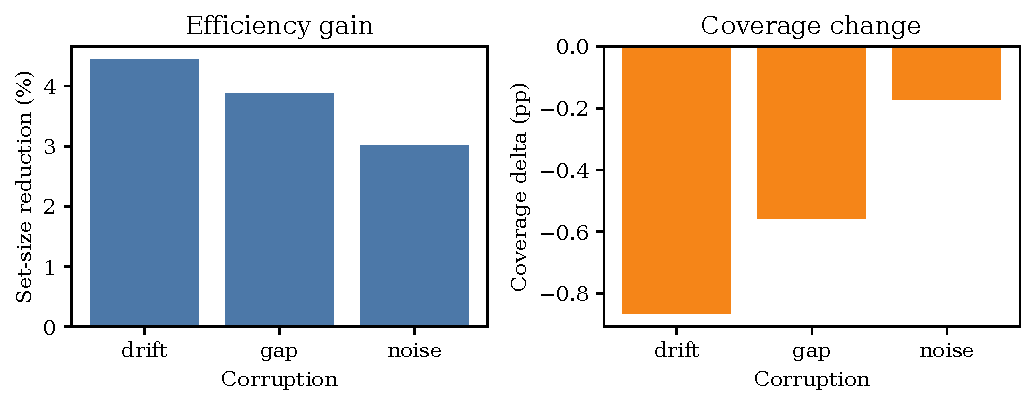
\includegraphics[width=0.95\linewidth]{figures/fig2_main_results.pdf}
    \caption{Expanded 35-dataset, five-seed benchmark at $\alpha=0.05$. \fastcp{}-efficient reduces prediction-set size relative to augmented split conformal prediction across drift, gap, and noise corruptions, with a small measured coverage decrease.}
    \label{fig:main_results}
\end{figure}

\Cref{fig:main_results} summarizes the main comparison from the expanded benchmark. \fastcp{}-efficient reduces average prediction-set size by 4.44\% under drift, 3.87\% under gaps, and 3.02\% under noise relative to augmented split conformal prediction. The corresponding coverage deltas are -0.0086, -0.0056, and -0.0017, respectively. Thus, the larger benchmark confirms a statistically significant efficiency gain, but also shows that the gain is not free: coverage decreases slightly on average, especially under drift.

The absolute coverage-gap delta is near zero under drift, slightly negative under gaps, and negative under noise. The overall mean absolute-gap delta is -0.0012 with a 95\% bootstrap confidence interval of [-0.0022, -0.0002]. We therefore frame the method as a significant set-size reduction with a small measured coverage tradeoff, not as a uniformly better calibrated method.

\begin{table}[t]
\centering
\small
\caption{Coverage-efficiency comparison under corrupted UCR evaluation. Size $\Delta$ is relative to augmented split conformal prediction. Positive values indicate smaller sets than Aug SCP, but should be interpreted jointly with coverage. \fastcp{}-efficient is a Pareto point, not a coverage-dominant method.}
\label{tab:full_method_table}
\resizebox{\linewidth}{!}{%
\begin{tabular}{lrrrrrrr}
\toprule
Method & Coverage & Set size & Abs. gap & Size $\Delta$ vs Aug & Drift size & Gap size & Noise size \\
\midrule
Clean SCP & 0.8656 & 1.9323 & 0.1049 & 0.4862 & 1.9412 & 1.9240 & 1.9315 \\
Aug SCP / global fallback & 0.9501 & 2.4185 & 0.0467 & 0.0000 & 2.4405 & 2.4151 & 2.3998 \\
APS & 0.9757 & 3.2595 & 0.0423 & -0.8411 & 3.2654 & 3.2128 & 3.3005 \\
RAPS & 0.9730 & 2.7313 & 0.0424 & -0.3128 & 2.7262 & 2.7293 & 2.7384 \\
Mondrian & 0.9553 & 2.5021 & 0.0418 & -0.0837 & 2.3172 & 2.7412 & 2.4480 \\
Conf-weighted & 0.9478 & 2.4262 & 0.0440 & -0.0078 & 2.4421 & 2.4310 & 2.4056 \\
\fastcp{}-local & 0.9440 & 2.3112 & 0.0446 & 0.1073 & 2.3003 & 2.3096 & 2.3236 \\
\fastcp{}-efficient & 0.9448 & 2.3254 & 0.0455 & 0.0931 & 2.3309 & 2.3240 & 2.3213 \\
\bottomrule
\end{tabular}
}
\end{table}

\subsection{Tail-risk analysis and deployment boundary}

\begin{figure}[t]
    \centering
    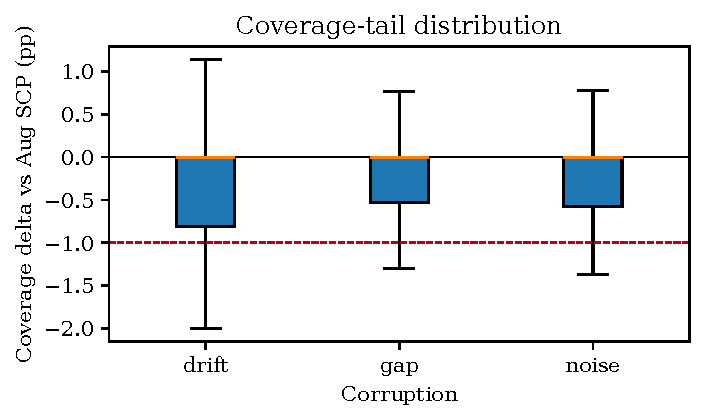
\includegraphics[width=0.62\linewidth]{figures/fig7_coverage_delta_tail.pdf}
    \caption{Distribution of coverage deltas for \fastcp{}-efficient relative to augmented split conformal prediction. The dashed line marks a one percentage point decrease.}
    \label{fig:coverage_tail}
\end{figure}

\begin{table}[t]
\centering
\small
\caption{Overall undercoverage tail-risk audit. Rates are fractions of the 1575 dataset/seed/corruption/severity evaluation cells.}
\label{tab:tail_risk}
\begin{tabular}{lrrrr}
\toprule
Method & Mean cov. & Below target & Below target -1pp & P10 cov. \\
\midrule
Aug SCP / global fallback & 0.9501 & 0.3283 & 0.2698 & 0.8777 \\
\fastcp{}-efficient & 0.9448 & 0.3905 & 0.3111 & 0.8699 \\
Confidence-only & 0.9494 & 0.3283 & 0.2660 & 0.8847 \\
\bottomrule
\end{tabular}
\end{table}

\Cref{fig:coverage_tail,tab:tail_risk} show the tail behavior behind the average tradeoff. \fastcp{}-efficient increases the overall fraction of evaluation cells below nominal coverage from 32.83\% to 39.05\%, and below nominal by more than one percentage point from 26.98\% to 31.11\%. The worst ten coverage drops are concentrated in very small test sets such as Coffee and BirdChicken, where one or two examples move empirical coverage substantially. Confidence-only weighting is safer in this audit, with mean coverage 0.9494 and a smaller undercoverage tail, but its prediction sets are much closer in size to augmented split conformal prediction.

\fastcp{}-efficient is therefore not recommended when coverage is a hard safety constraint. In such settings, the coverage-prioritized mode should be used; on this benchmark that mode falls back to the augmented global threshold. This is the intended deployment boundary of the local-global family rather than an exception to the method.

\subsection{Severity-level analysis}

\begin{table}[t]
\centering
\small
\caption{Severity-level behavior averaged over gap, noise, and drift corruptions. Low, medium, and high correspond to the three severity levels within each corruption family.}
\label{tab:severity_summary}
\begin{tabular}{lrrrr}
\toprule
Severity & Aug cov. & FAST cov. & Cov. delta & Set reduction \\
\midrule
Low & 0.9774 & 0.9730 & -0.0044 & 0.1115 \\
Medium & 0.9671 & 0.9607 & -0.0064 & 0.1017 \\
High & 0.9058 & 0.9007 & -0.0052 & 0.0661 \\
\bottomrule
\end{tabular}
\end{table}

\Cref{tab:severity_summary} shows that severe corruptions are difficult for both methods: augmented split conformal prediction already falls to 0.9058 mean coverage at the high severity level. The FAST-CP coverage drop remains on the same order across severities, while the set-size reduction becomes smaller under high severity. The practical use case of \fastcp{}-efficient is therefore low-to-moderate corruption, where the global threshold is not already severely strained. Under severe corruptions, users should prefer validation-selected global fallback behavior.

\subsection{External multivariate validation}

To reduce dependence on univariate UCR evidence, we add a small external validation on three UEA multivariate datasets: BasicMotions, Epilepsy, and NATOPS. These datasets contain real multichannel sensor or motion signals; we evaluate them under synthetic gap, noise, and drift stress tests. The run uses three seeds, $\alpha=0.05$, 24 random convolution kernels per channel, and the same augmented calibration pool and $\lambda=0.35$ mixed threshold.

\begin{table}[t]
\centering
\small
\caption{External UEA multivariate validation. Values compare the mixed FAST-CP setting with augmented split conformal prediction across 81 dataset/seed/corruption/severity cells.}
\label{tab:uea_external}
\begin{tabular}{lrrrr}
\toprule
Corruption & FAST cov. & Aug cov. & Cov. delta & Set reduction \\
\midrule
Drift & 0.9499 & 0.9519 & -0.0019 & 0.0441 \\
Gap & 0.9491 & 0.9479 & 0.0012 & 0.0527 \\
Noise & 0.9639 & 0.9658 & -0.0019 & 0.0542 \\
Overall & 0.9543 & 0.9552 & -0.0009 & 0.0503 \\
\bottomrule
\end{tabular}
\end{table}

\Cref{tab:uea_external} gives a small but useful external check. The set-size reduction remains positive across all three corruption families, while the overall coverage delta is -0.0009 and its bootstrap confidence interval includes zero. This does not replace real corrupted deployment data, but it shows that the basic tradeoff is not limited to univariate UCR series.

\subsection{Local-global mix ablation}

\begin{figure}[t]
    \centering
    
\includegraphics[width=0.58\linewidth]{figures/fig3_mix_ablation.pdf}
    \caption{Ablation of the local-global threshold mix on five datasets. Intermediate mixing recovers coverage relative to purely local thresholds while retaining smaller prediction sets than the global augmented threshold.}
    \label{fig:mix_ablation}
\end{figure}

\Cref{fig:mix_ablation} shows that the mixing coefficient is not merely cosmetic. Pure local weighting gives smaller sets but weaker coverage behavior, while $\lambda=1$ recovers augmented split conformal prediction with larger sets. Intermediate values, particularly 0.2 and 0.35, provide practical tradeoff points on the ablation subset.

\subsection{Validation of safe fallback and Pareto operating points}

\begin{figure}[t]
    \centering
    
\includegraphics[width=0.95\linewidth]{figures/fig6_lambda_pareto.pdf}
    \caption{Held-out alpha/lambda Pareto analysis over 25 evaluation datasets. Each panel averages over corruption families and plots the local-global threshold path from pure local weighting ($\lambda=0$) to augmented split conformal prediction ($\lambda=1$, labeled as Aug SCP).}
    \label{fig:lambda_pareto}
\end{figure}

To validate the two-mode protocol, we split the 35 valid UCR datasets into 10 tuning datasets and 25 held-out evaluation datasets. On the tuning split, we evaluate $\lambda\in\{0,0.1,0.2,0.35,0.5,0.65,0.8,1\}$ at $\alpha\in\{0.05,0.1,0.2\}$ with three seeds. A lambda is considered feasible only if its mean coverage is at least $1-\alpha-0.01$ for every alpha; among feasible lambdas, the rule chooses the smallest average set size.

No lambda satisfied this feasibility rule on the tuning split. The fallback rule, which minimizes total coverage shortfall and then set size, selected $\lambda=1$, equivalent to augmented split conformal prediction. This result confirms the need to distinguish the two operating modes. When coverage is prioritized, the validation protocol selects the global augmented threshold. When efficiency is prioritized, intermediate $\lambda$ values define Pareto points with measurable set-size reductions and explicit coverage costs.

\Cref{fig:lambda_pareto} summarizes the held-out Pareto behavior. At $\alpha=0.05$, $\lambda=0.35$ reduces average set size by 0.1125 labels relative to $\lambda=1$ with a 95\% bootstrap confidence interval of [0.0997, 0.1269], but lowers coverage by 0.0083. At $\alpha=0.10$, the reduction decreases to 0.0392 labels with a coverage delta of -0.0052. At $\alpha=0.20$, the reduction is only 0.0109 labels and the coverage delta is not statistically clear. Thus, local weighting is most useful at stricter coverage levels, while broader alpha settings make the efficiency advantage much smaller.

\begin{table}[t]
\centering
\small
\caption{Held-out tradeoff of $\lambda=0.35$ relative to $\lambda=1$ (Aug SCP) across target miscoverage levels.}
\label{tab:lambda_tradeoff}
\begin{tabular}{lrrrr}
\toprule
$\alpha$ & Set reduction & 95\% CI & Coverage delta & 95\% CI \\
\midrule
0.05 & 0.1125 & [0.0997, 0.1269] & -0.0083 & [-0.0109, -0.0058] \\
0.10 & 0.0392 & [0.0296, 0.0499] & -0.0052 & [-0.0083, -0.0026] \\
0.20 & 0.0109 & [0.0046, 0.0179] & -0.0009 & [-0.0032, 0.0012] \\
\bottomrule
\end{tabular}
\end{table}

\subsection{MiniROCKET backbone check}

As a stronger-backbone supplement, we repeat the evaluation on 15 fixed UCR datasets with MiniROCKET features and a calibrated ridge classifier. The run uses three seeds, $\alpha\in\{0.05,0.10\}$, and the same gap, noise, and drift corruptions. Compared with $\lambda=1$, the $\lambda=0.35$ mixed threshold reduces average set size by 0.0943 labels at $\alpha=0.05$ with a 95\% confidence interval of [0.0770, 0.1121], while decreasing coverage by 0.0055. At $\alpha=0.10$, it reduces set size by 0.0694 labels with a 95\% confidence interval of [0.0559, 0.0833], while decreasing coverage by 0.0067. The qualitative tradeoff therefore persists under a stronger MiniROCKET-based classifier, although this does not establish transfer to deep InceptionTime, ResNet, or transformer backbones.

\subsection{FCN backbone check}

We also run a small deep-backbone check with an FCN classifier on eight representative UCR datasets: ECG200, GunPoint, Coffee, BME, FaceFour, ItalyPowerDemand, MoteStrain, and Beef. The run uses two seeds, 20 epochs, $\alpha=0.05$, and the same gap, noise, and drift corruptions. This is not a full deep TSC benchmark, but it directly tests whether the mixed-threshold behavior disappears once the base classifier is no longer a linear model over random features.

\begin{table}[t]
\centering
\small
\caption{Small FCN backbone check. Values compare the mixed FAST-CP setting with augmented split conformal prediction across 144 dataset/seed/corruption/severity cells.}
\label{tab:fcn_backbone}
\begin{tabular}{lrrrr}
\toprule
Corruption & FAST cov. & Aug cov. & Cov. delta & Set reduction \\
\midrule
Drift & 0.9519 & 0.9544 & -0.0026 & 0.0139 \\
Gap & 0.9426 & 0.9431 & -0.0005 & 0.0139 \\
Noise & 0.9679 & 0.9691 & -0.0012 & 0.0138 \\
Overall & 0.9541 & 0.9556 & -0.0014 & 0.0139 \\
\bottomrule
\end{tabular}
\end{table}

\Cref{tab:fcn_backbone} shows a smaller but consistent efficiency gain under FCN. The overall set-size reduction is 0.0139 labels with a 95\% bootstrap confidence interval of [0.0090, 0.0194], while the coverage delta is -0.0014 with a 95\% interval of [-0.0024, -0.0006]. This supports the narrower claim that the Pareto behavior is not exclusive to the compact baseline, while leaving larger InceptionTime, ResNet-style, and transformer TSC evaluations as future work.

\subsection{Dataset-level behavior}

\begin{figure}[t]
    \centering
    
\includegraphics[width=0.58\linewidth]{figures/fig4_win_loss.pdf}
    \caption{Dataset/seed/corruption-level comparison of \fastcp{}-efficient against augmented split conformal prediction.}
    \label{fig:win_loss}
\end{figure}

At the dataset/seed/corruption/severity level, \fastcp{}-efficient obtains a set-size win rate of 71.30\%. Its coverage is within one percentage point of augmented split conformal prediction in 73.33\% of comparison cells, and its absolute coverage-gap win rate is 82.48\%. These results show that the aggregate gains are not driven solely by one corruption type, although several datasets remain unfavorable for set-size reduction.

\subsection{Statistical tests and stronger baselines}

Paired tests over 1575 evaluation cells confirm that the set-size reduction against augmented split conformal prediction is statistically significant: the overall mean reduction is 0.0931 labels with a 95\% bootstrap confidence interval of [0.0856, 0.1007], and the Wilcoxon test gives $p<10^{-100}$. However, the same paired analysis shows a significant mean coverage decrease of -0.0053. Against APS and RAPS, \fastcp{}-efficient produces much smaller sets, but with larger coverage drops; these baselines are more conservative on this benchmark. Against the corruption-family Mondrian baseline, \fastcp{}-efficient has smaller sets overall but worse coverage and absolute-gap behavior under gap and noise. This comparison makes the tradeoff explicit: the method is efficient, but not uniformly dominant.

\subsection{Fingerprint ablations}

\begin{table}[t]
\centering
\small
\caption{Fingerprint contribution audit under the same mixed-threshold framework. All variants use the augmented calibration pool and $\lambda=0.35$; size $\Delta$ is measured against augmented split conformal prediction.}
\label{tab:fingerprint_variants}
\begin{tabular}{lrrrr}
\toprule
Variant & Coverage & Set size & Abs. gap & Size $\Delta$ \\
\midrule
Random fingerprint & 0.9440 & 2.3681 & 0.0489 & 0.0504 \\
Input-only & 0.9387 & 2.2820 & 0.0474 & 0.1365 \\
Confidence-only & 0.9494 & 2.3921 & 0.0443 & 0.0263 \\
Full fingerprint & 0.9448 & 2.3254 & 0.0455 & 0.0931 \\
\bottomrule
\end{tabular}
\end{table}

\Cref{tab:fingerprint_variants} clarifies the role of the fingerprint. The gain of \fastcp{} comes from two sources: local-threshold variability induced by the mixed conformal family, and meaningful perturbation-aware weighting. The random-fingerprint control shows that the threshold family itself can reduce set size, whereas the confidence-only and input-only variants reveal different risk-efficiency regimes. Input-only descriptors are aggressive, reducing set size by 0.1365 labels but lowering mean coverage to 0.9387. Confidence-only weighting is safer, with mean coverage 0.9494 and the smallest undercoverage tail, but it gives only a 0.0263-label set-size reduction. The full fingerprint is not coverage-dominant, but it provides a middle-ground tradeoff: larger efficiency gain than confidence-only weighting and less coverage degradation than input-only descriptors.
